\section{Experiments}
In this section we first present our experiments setup and baseline models in \secref{sec:exp} and \secref{sec:baseline} respectively. Then we show the different aspects of evaluation results and give a detailed analysis from \secref{sec:ana} to \secref{sec:ga}. According to our experiments, we want to determine these questions: First, does the maximum margin function help to automatically generate templates and does dynamic demonstration work in the few-shot setting? Second, are the sentences produced by our model reasonable? Third, how is the generalization ability of our dynamic demonstration method?

\subsection{Experiments Setup}
\noindent
\textbf{Dataset.} We evaluate our model on two English datasets: SNLI and MNLI. Because the MNLI test set doesn't have ground truth labels, we use the mismatched development set as the test set and matched development set as the development set. Different from~\citet{DBLP:conf/acl/GaoFC20} use $K=16$ for classification tasks, we set $K=200$ considering the generation task is more challenging. Detailed statistics are listed in \tabref{table:dataset}. 
\label{sec:exp}
\begin{table}[!h]
	\centering
	\small
	\begin{tabular}{l|ccc}
		\toprule
		\textbf{Dataset} & \textbf{\#Training} & \textbf{\#Development} & \textbf{\#Test}\\
		\midrule
		SNLI  & 550,152 &  10,000 & 10,000 \\
		MNLI   & 392,302 &  10,000 & 10,000 \\
		\bottomrule
	\end{tabular}
	\caption{Statistics of SNLI and MNLI dataset.}
	\label{table:dataset}
\end{table}

\begin{table*}[t!]
	% \renewcommand\arraystretch{1.3}
	\setlength\tabcolsep{4pt}
	\centering
	\small
	\begin{tabular}{l|cccccc|cccccc}
		\toprule
		\multirow{2}{*}{\textbf{Methods}} & \multicolumn{6}{c|}{\textbf{SNLI}} &\multicolumn{6}{c}{\textbf{MNLI}}  \\
		
		&\textbf{acc~(\%)}   &\textbf{B-4}  &\textbf{R-2}  &\textbf{PPL$\downarrow$}    &\textbf{Div-2}  &\textbf{Div-3}  &\textbf{acc~(\%)}   &\textbf{B-4}  &\textbf{R-2}  &\textbf{PPL$\downarrow$}     &\textbf{Div-2}  &\textbf{Div-3}   \\
		\midrule
		% \textbf{\textit{Full-shot}} & & & & & & & & & & & & & & \\
		% \midrule 
		BART-large$^\spadesuit$  & 94.17 & 8.75 & 17.63&41.91 &0.214 &0.407 &89.42 &10.55 &19.25 & 39.74& 0.365& 0.570\\
		\midrule
		% \textbf{\textit{Zero-shot}}  & & & & & & & & & & & & & & \\
		% \midrule
		Rule-base$^\clubsuit$  & 75.30 & 5.13 & 12.83 & 114.34 & 0.213& 0.402&69.07 &6.44 &16.45 &107.18 &0.289 &0.467 \\
		\midrule
		% \textbf{\textit{Few-shot}}  & & & & & & & & & & & & & & \\
		% \midrule
		AMD  & 34.75(1.91) & 0.81 & 2.19 & 678.45 & 0.097& 0.265& 34.66(3.16)&0.00 &0.25 &981.49 &0.198 & 0.547\\
		BART-large  & 66.45(8.00) & 8.63 & 15.27 &\textbf{61.93} &0.182 &0.356 &55.45(4.33) &\textbf{10.05} &16.69 &\textbf{45.35} &0.415 &0.640 \\
		\midrule
		$Prompt_{man}$ & 67.41(5.63) & 8.63 &15.58 & 67.49& 0.176& 0.343& 58.62(3.01)&9.66 &16.57 &47.46 &0.424 &0.649 \\
		$\ +static$ & 71.13(9.44) & \textbf{9.10} &\textbf{15.93} &63.95 &0.176 &0.342 &59.82(5.66) &9.90 &16.58 &47.47 &0.426 &0.650 \\
		$\ +dynamic$ & 74.01(7.89) & 8.11 &14.58 &71.36 &0.188 &0.362 &\textbf{63.33}(1.97) &9.35 &16.10 &48.87 &\textbf{0.442} &\textbf{0.674}  \\
		\midrule
		$Prompt_{top}$ & 68.04(10.01)& 8.50& 15.38& 67.79&0.176 &0.344 &59.20(9.81) &9.64 &16.45 &47.64 &0.425 &0.653 \\
		$\ +static$ & 66.79(12.23) &8.08 & 14.71& 63.57& 0.174& 0.336& 59.39(5.34)& 9.96& \textbf{16.71}& 46.39 & 0.426& 0.649\\
		$\ +dynamic$ & 73.69(4.16) & 8.10& 14.49& 68.72& 0.191& 0.367& 62.57(4.30)& 9.54& 16.29& 47.42& 0.434& 0.662\\
		\midrule
		$Prompt_{mm}$ & 69.33(6.82) & 8.51 &15.53 & 67.79& 0.176& 0.345& 59.53(4.20)&9.75 &\textbf{16.71} &47.64 &0.423 &0.647 \\
		$\ +static$ & 71.81(6.17) &8.71 & 15.49& 65.39& 0.177& 0.342& 59.78(4.33)& 9.69& 16.36& 46.60& 0.424& 0.647\\
		$\ +dynamic$ & \textbf{74.44}(4.74) & 7.97&14.42 &70.28 &\textbf{0.192} &\textbf{0.370} &62.57(2.13) &9.38 &16.04 &47.45 &0.440 &0.670 \\
		\bottomrule
	\end{tabular}
	\caption{Our main results using BART-large generator. Best results in few-shot settings are marked with \textbf{bold} font. $\spadesuit$ stands for \textbf{\textit{Full-shot}}: fine-tune with full data; $\clubsuit$  stands for \textbf{\textit{Zero-shot}}: no training data; other methods are in \textbf{\textit{Few-shot}} setting: we use $K$ = 200 (per class) for few-shot experiments. We report mean performance over 5 different split. For accuracy metric, we also report standard deviation; $man$: use manually defined prompt; $top$: auto prompt selected by maximum score; $mm$: auto prompt selected by max margin; $static$: use static SBERT as the retriever; $dynamic$: train SBERT retriever with generator; $\downarrow$:lower is better.}
	\label{table:linkprediction}
\end{table*}

\noindent
\textbf{Evaluation Metrics.} We adopt the standard text generation metrics perplexity (PPL), BLEU-4 score~\citep{papineni2002bleu} and ROUGE-2 score~\citep{lin-2004-rouge} to automatically compare generated results and reference hypotheses. Since these metrics do not consider the semantic meaning of sentences, we further use a state-of-the-art NLI classifier trained on 4 datasets~\citep{nie-etal-2020-adversarial} to calculate the accuracy of predictions, which achieves 92.6\% and 90.6\% accuracy in SNLI and MNLI mismatched datasets respectively. Good hypotheses are supposed to be not only accurate but also diverse, and therefore we use distinct n-grams normalized by the total number of generated n-grams Div-n~\citep{li-etal-2016-diversity} to measure diversity.
We also develop human evaluation in~\secref{sec:he}.

\noindent
\textbf{Implement Details.} We use BART-large as the generator. For the retriever, we deploy our experiment with the BERT-base and SBERT models. We optimize models using Adam~\citep{DBLP:journals/corr/KingmaB14}. The hyper-parameters are chosen by $\mathcal{D}_{dev}$. The max length is set to 128 for non-demonstration methods and 170 for others. We conduct all experiments on single NIVIDIA V100 16GB GPUs without half-precision. We use ROUGE-2 on the development set to choose the best models instead of the accuracy because we find the NLI classifier tends to give high accuracy even before the model is converged. More details can be found in Appendix A and B, including the generality of dynamic demonstration and generated prompts.

\subsection{Baselines}
\label{sec:baseline}
We compare our model with both unsupervised and supervised methods:

\noindent
\textbf{Rule-base:} A simple rule-based method. First, we use Stanford Stanza~\citep{qi2020stanza} to tokenize premises and get POS tags. For entailment, we simplify the premises by removing \textbf{\textit{adj}} and \textbf{\textit{adv}} words as hypothesis. For contradiction, we randomly replace one word in each premise with its antonym. If there are no candidate words, we add negative words into the sentence (e.g. ``not'' and ``don't''). For neutral, we randomly replace one word in each premise with its hyponym.

\noindent
\textbf{AMD:} A RNN-based model proposed by ~\citet{DBLP:journals/csl/StarcM17}. It learns a latent representation $\mathbf{z}$ that represents the mapping between the premise and the
label on one side, and the hypothesis on the other side.

\noindent
\textbf{BART-large:} A pre-trained language model which performances well on a range of abstractive dialogue, question answering, and summarization tasks.

\subsection{Main Results \& Analysis}
\label{sec:ana}
Our main results is shown in \tabref{table:linkprediction}. Overall, the full-shot finetuning of the BART-large model performs best except for diversity with overwhelming training consumption as a sacrifice, and the rule-base method outperforms methods in few-shot settings in terms of accuracy, while fails to perform well in other metrics. Despite the fair accuracy, the rigid rule leads the generated hypotheses less comprehensible, and the trivial edition would not provide much gain for data augmentation. In the few-shot setting, AMD is poor due to lack of pre-trained knowledge, and prompt-based methods take advantage over the most of metrics because the training and the predicting share the same LM objective. 
Generally, the B-4, R-2 and PPL are not always consistent with the accuracy result but the oscillation is slight. The increase of diversity is usually associated with the decline of B-4 and R-2, which is explainable because these metrics only consider the overlap of n-grams with one fixed reference sentence and neglect their semantic meaning. Our dynamic demonstration yields the best accuracy score in few-shot settings, achieving 8\% improvement over BART-large model in both SNLI and MNLI datasets. The diversity of our methods even exceeds BART-large trained in the full-shot scenario on MNLI, which is meaningful for the data augmentation application. 

\noindent
\textbf{Prompt Template Selection.}
When comparing different prompt generation strategies $man$, $top$ and $mm$ without demonstrations, we can find the manually designed prompt performs not as good as prompts generated by T5 model in accuracy and diversity metric, and for the accuracy of automatic generation prompts, those selected by max-margin function beat those selected by maximum score on most of metrics. This verifies our assumption that good templates of one condition get high scores in the corresponding condition while low in other conditions, and good templates narrow down the standard deviation of the accuracy.

\noindent
\textbf{Demonstration Selection.}
Under each prompt generation setting, we observe that the static demonstration improves the most of results over the original prompt except the $top$ setting, mainly due to the instability of templates generated by the maximum score. Our proposed dynamic demonstration method boosts the accuracy and diversity result with considerable gain, including the $top$ setting, which indicates that our dynamic demonstration is able to distinguish the more proper demonstration example. On the MNLI dataset, the dynamic demonstration achieves the best accuracy on manually defined templates, reflecting that in some cases the manual prompt template is simple but effective when the number of conditions is limited. In general, the dynamic demonstration shows its competitiveness no matter which prompt template selection strategy is.

\subsection{Human evaluation}
\label{sec:he}
In order to check the quality of the generated hypotheses, we carry out human evaluation. We recruit 5 students who are proficient in English to score the generation result of six models, with 50 samples in each condition and each dataset, and each sample is labeled by at least 3 evaluators. We examine two aspects of the quality: (1) Is the hypothesis in the right condition with the premise? (0 or 1) (2) Is the sentence reasonable grammatically? (0, 1 or 2, the higher the better). The main result is illustrated in the first two subfigures in \figref{fig:human}. For accuracy, the max-margin strategy is helpful in static demonstration, but in SNLI's dynamic demonstration things are different, maybe the power of dynamic demonstration hides the advantage of max-margin. The improvement of dynamic demonstration is always eye catching, which is consistent with auto-metric in \tabref{table:linkprediction}. For grammaticality, the rule-based method is inferior to other methods, indicating that the rule-based method owns poor readability despite the accuracy.

\begin{figure}[th]
	\centering
	\scalebox{1.0}{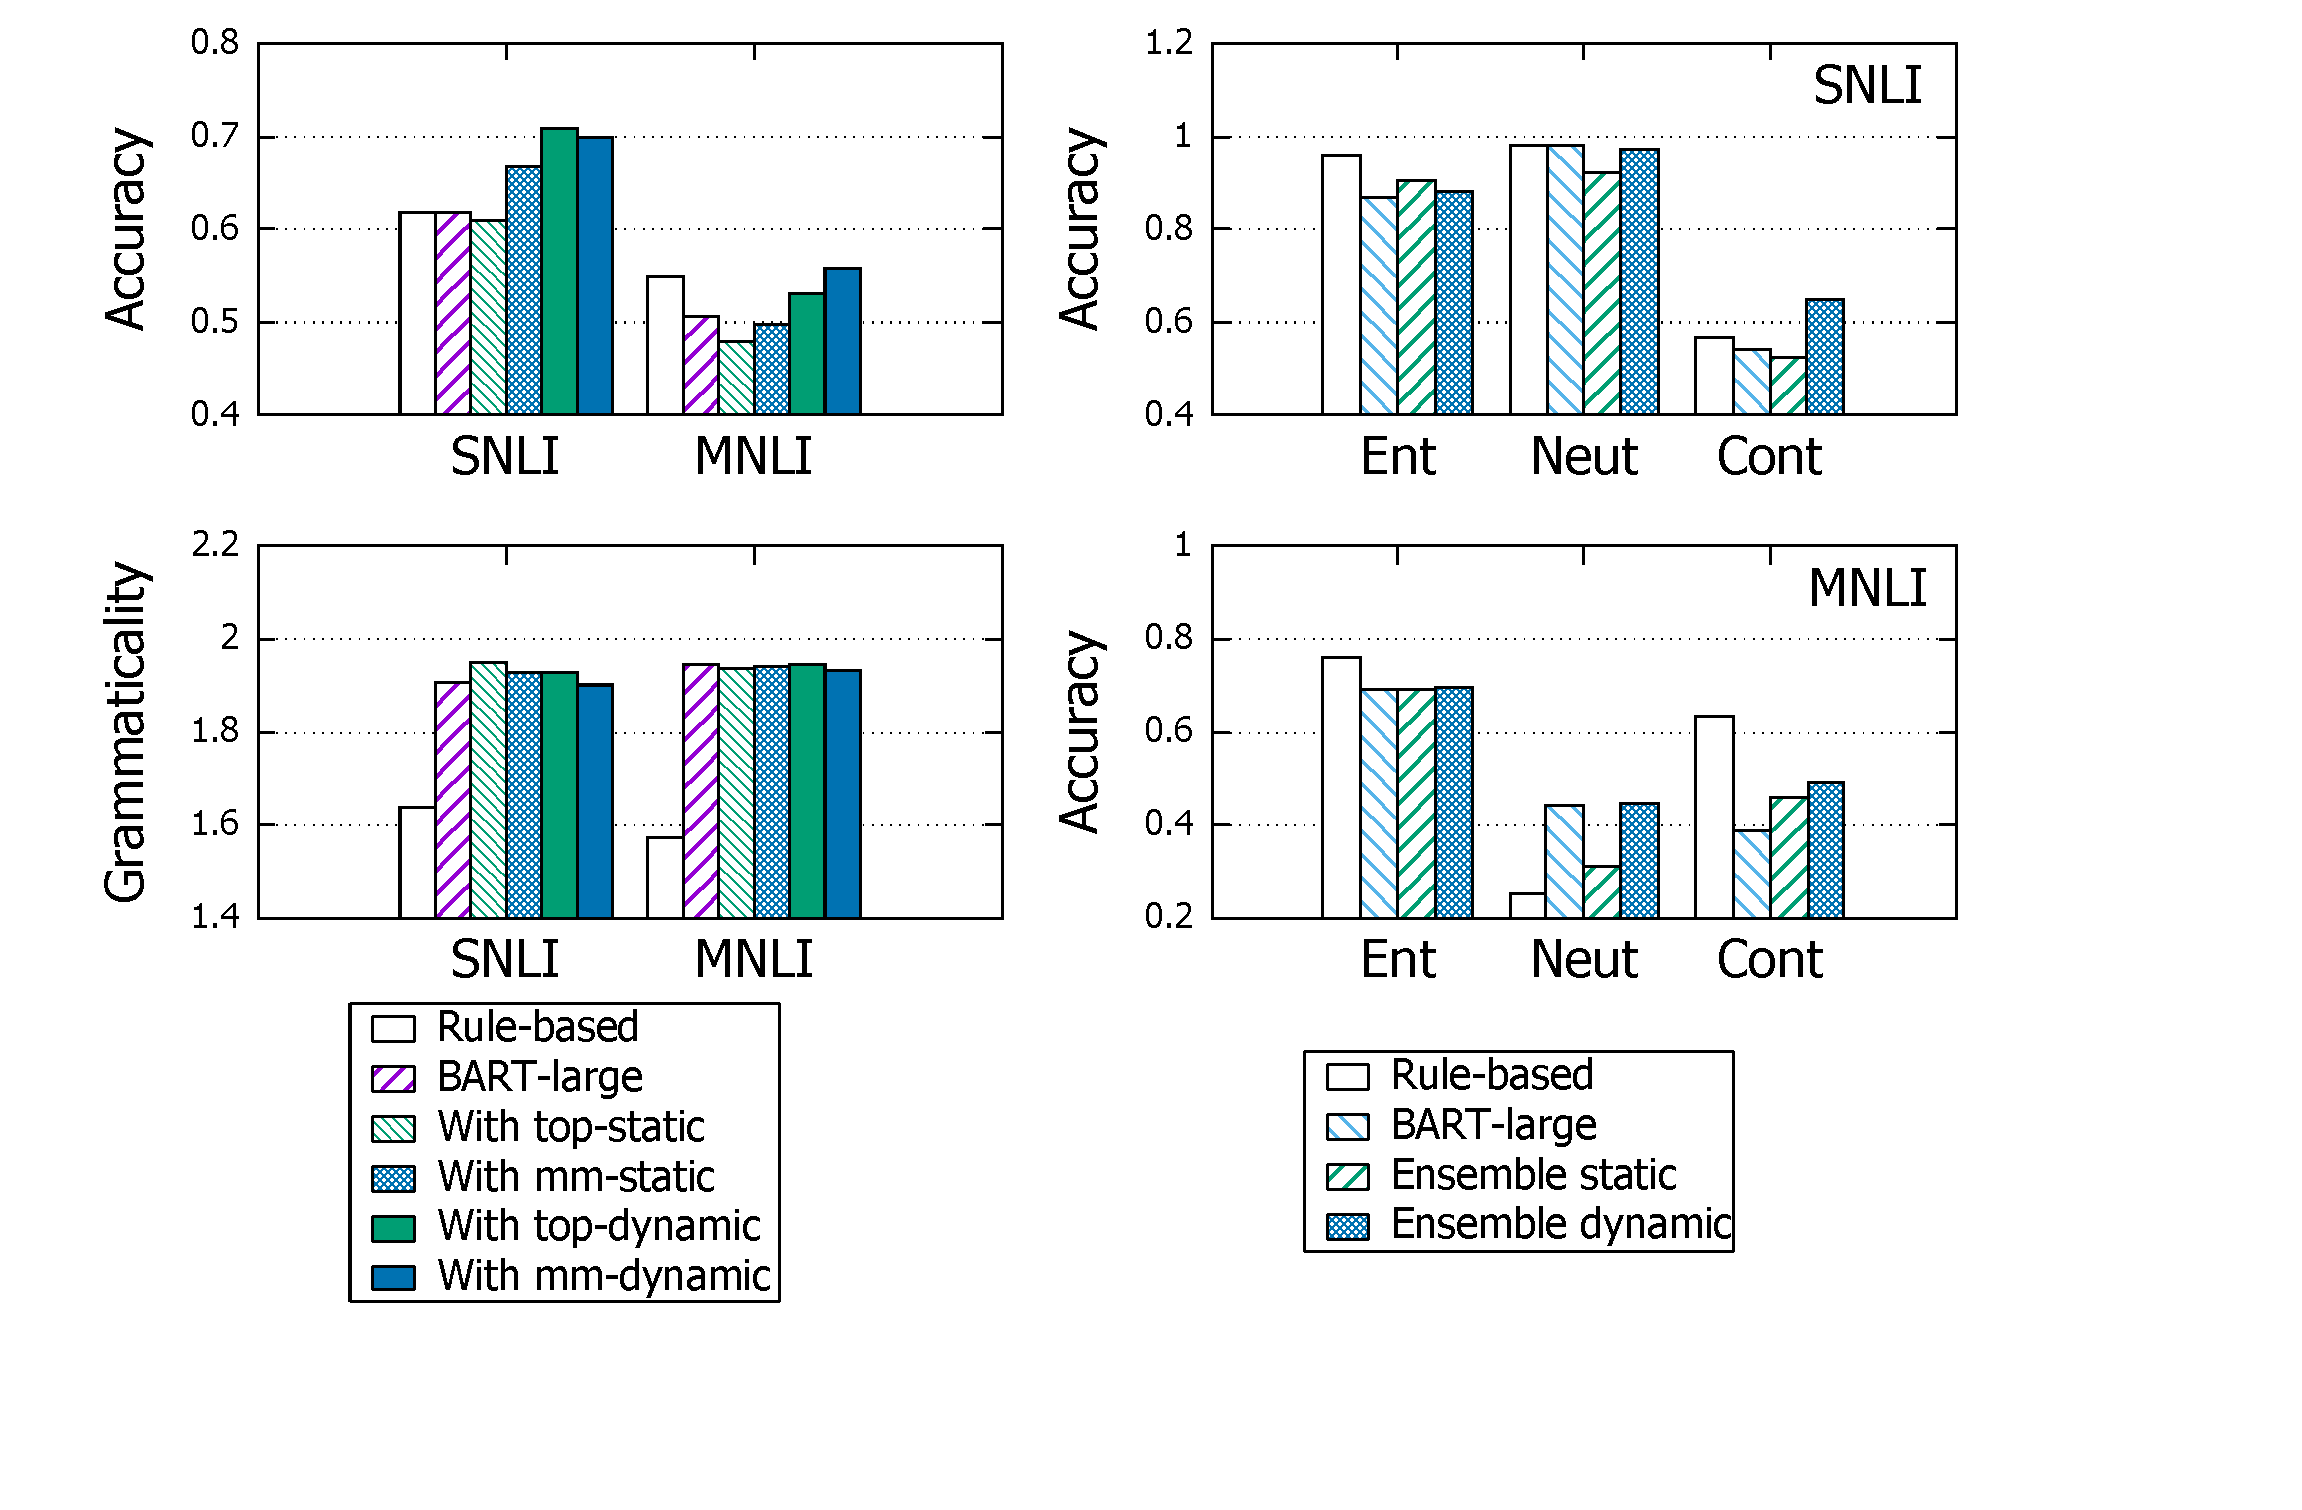
\includegraphics[width=1\columnwidth]{figure/human.pdf}}
	\caption{First column: the human evaluation of different datasets. The same color stands for the same prompt selection. Second row: accuracy of entailment, neutral and contradiction respectively, and here we merge the results of static and dynamic demonstration of different prompt selection methods as the ensemble results.}
	\label{fig:human}
\end{figure}

To further investigate the power of dynamic demonstration in different conditions, we can find that the advantage is not obvious under the scenario where these methods already obtain high accuracy, like entailment. Instead, it is more facilitative under those difficult conditions.


% 		Bart-large \\
%\textbf{Input:} A young family enjoys feeling ocean waves lap at\\ 
%their feet. \\
%\textbf{condition:} contradiction \\
%\textbf{Output:} The ocean.\\
%\textbf{Classifier output:} Entailment \\

\subsection{Case study}
The case study result is shown in \tabref{table:case}. For the static method, it finds the simple connection between ``family'' and ``child'' while fails to recognize the semantic relation between the demonstration and the premise. For the dynamic method, in addition to finding the connection between ``ocean'' and ``beach'', it also excavates the deeper pattern, which helps the PLM to generate the correct corresponding hypothesis. 
The case shows our dynamic demonstration method can find a more similar example as a demonstration to guide the generation than the static method.

\begin{table}[!h]
	\centering
	\small
	\begin{tabular}{l}
		\toprule
		SBERT + static \\
	   \textbf{Input:} \underline{A child playing with a sword at the bottom of the} \\
	   \underline{stairs. \textcolor{blue}{As} a child playing with a spoon.} [SEP] A young \\
	   family enjoys feeling ocean waves lap at their feet. \textcolor{blue}{As}\_\_\\ 
	   \textbf{condition:} Contradiction \\
	   \textbf{Output:}  The waves are crashing onto the beach..\\
	   \textbf{Classifier output:} Neutral (Bad generation)\\
		\\
		SBERT + dynamic \\
		\textbf{Input:} \underline{A middle-aged woman in a dark bathing suit and} \\\underline{her middle-aged husband in an orange hat walk cozily} \\ \underline{along the beach. \textcolor{blue}{As} there is no water.} [SEP] A young \\ family enjoys feeling ocean waves lap at their feet. \textcolor{blue}{As}\_\_\\ 
		\textbf{condition:} Contradiction \\
		\textbf{Output:}  There is no sand.\\
		\textbf{Classifier output:} Contradiction (Good generation)\\
		\bottomrule
	\end{tabular}
	\caption{Case study for the dynamic method. The underline text is demonstrations. Template words are marked as blue.}
	\label{table:case}
\end{table}
% %		Bart-large & A group of people dancing together. & A group of people is dancing. & N & E\\
%%		\midrule
%%		SBERT + dynamic & 
%\tabincell{l}{\underline{Four girls are standing together in their dance outfits.} \\\underline{\textcolor{blue}{Later,} four girls are at a dance.} [SEP] A group of \\people dancing together. \textcolor{blue}{Later,} } & A group of people are dancing. & Neutral & Entailment\\

\subsection{Generality test}
\label{sec:ga}
In order to evaluate the generality of our dynamic demonstration 
method, we implement it based on state-of-the-art few-shot approach: LM-BFF 
and develop experiments on 13 NLP classification tasks.
We use $K=10$ for all the tasks.
The LM-BFF implemented by ourselves uses the same setting in the original paper. In few-shot settings, the performance of model suffers from instability, and our implementing results are quite different from theirs\footnote{We directly run their released code from: \url{https://github.com/princeton-nlp/LM-BFF}}, so we only compare with our implementing results. As shown in table \ref{table:generazation}, our dynamic demonstration method outperforms the static method on 10 out of 13 tasks, which suggests its strong generality. 

Besides, during the test, LM-BFF samples demonstration sets from $D_{train}^{'}$ and ensemble the predictions across all sets, while for our dynamic demonstration, we abandon it because our dynamic demonstration method has the ability to tune hidden vectors on $D_{train}^{'}$ during training, and the model is expected to have the best result with the top-1 example, so there is no need to ensemble model to make the results more stable.

\begin{table}[!h]
	\centering
	\small
	\begin{tabular}{l|cc}
		\toprule
		 & \textbf{Training} & \textbf{Inference}\\
		\midrule
		LM-BFF  & 10x &  1x \\
		LM-BFF+dynamic   & 1x &  16x \\
		\bottomrule
	\end{tabular}
	\caption{Training and inference speed comparison}
	\label{table:time}
\end{table}

Table \ref{table:time} is a comparison of training and inference speed. We can see our dynamic method takes more time to train dynamic demonstration while it takes less time to do inference. The training speed for dynamic demonstration directly depends on the hyper parameter $K$, and under the few-shot setting, a small $K$ guarantees the training speed would not be too slow.

\begin{table*}[th]
	\centering
	\small
	\begin{tabular}{l|ccccccc}
		\toprule
		 & \textbf{SST-2} & \textbf{SST-5} & \textbf{MR} & \textbf{CR} & \textbf{MPQA} & \textbf{Subj} & \textbf{TREC} \\
		\midrule
		\textbf{LM-BFF} (In paper)  & 93.0(0.6) & 49.5(1.7) & 87.7(1.4) & 91.0(0.9) & 86.5(2.6) & 91.4(1.8) & 89.4(1.7) \\
		\midrule 
		\textbf{LM-BFF} (Our implement)   & \textbf{93.0}(0.5) & 50.4(1.2) & 87.3(1.9) & 90.7(1.1) & 86.2(1.8) & 90.4(2.3) & 86.2(3.9)\\
		\textbf{LM-BFF}$+dynamic$ & 91.8(0.9) & \textbf{50.6}(1.3)& \textbf{88.0}(1.1) & \textbf{91.2}(0.8) & \textbf{86.7}(1.7) & \textbf{91.2}(1.7) & \textbf{87.3}(3.0) \\
		\midrule 
		 & \textbf{CoLA} & \textbf{SNLI} & \textbf{QNLI} & \textbf{RTE} & \textbf{MRPC} & \textbf{QQP} & \textbf{-}\\
		\midrule 
		\textbf{LM-BFF} (In paper)  & 21.8(15.9) & 77.5(3.5) & 68.5(5.4) & 71.1(5.3) & 78.1(3.4) & 67.7(5.8) &\textbf{-}\\
		\midrule 
		\textbf{LM-BFF} (Our implement)   & \textbf{20.4}(14.4)& \textbf{80.5}(1.7)& 70.5(4.8) & 69.0(3.3) & 75.0(4.5) &58.6(6.4)&\textbf{-}\\
		\textbf{LM-BFF} $+ dynamic$ & 17.7(17.5) & 78.9(2.4) & \textbf{71.9}(3.7) & \textbf{72.5}(3.7) & \textbf{77.4}(3.8) & \textbf{66.4}(7.4) &\textbf{-}\\
		\bottomrule
	\end{tabular}
	\caption{Test dynamic demonstration method on 13 NLP classification tasks. }
	\label{table:generazation}
\end{table*}

